\documentclass[
	letterpaper, % Paper size, specify a4paper (A4) or letterpaper (US letter)
	10pt, % Default font size, specify 10pt, 11pt or 12pt
]{CSUniSchoolLabReport}

\usepackage{fancyvrb}

% redefine \VerbatimInput
\RecustomVerbatimCommand{\VerbatimInput}{VerbatimInput}%
{fontsize=\footnotesize,
 %
 frame=lines,  % top and bottom rule only
 framesep=2em, % separation between frame and text
 rulecolor=\color{Gray},
 %
 label=\fbox{\color{Black} Power Flow Solution — Base Case}, 
 labelposition=topline,
 %
 commandchars=\|\(\), % escape character and argument delimiters for
                      % commands within the verbatim
 commentchar=*        % comment character
}

%----------------------------------------------------------------------------------------
%	REPORT INFORMATION
%----------------------------------------------------------------------------------------

\title{Lab Six (Part B)\\ Power Systems Analysis \\ EECE5682} % Report title

\author{Michael \textsc{Brodskiy}\\ \small \href{mailto:Brodskiy.M@Northeastern.edu}{Brodskiy.M@Northeastern.edu}}

\date{November 20, 2024} % Date of the report

%----------------------------------------------------------------------------------------


\begin{document}

\maketitle % Insert the title, author and date using the information specified above

\begin{center}
	\begin{tabular}{l r}
		Date Performed: & \today \\ % Date the experiment was performed
		Instructor: & Professor \textsc{Abur} \\ % Instructor/supervisor
	\end{tabular}
\end{center}

\newpage

\begin{abstract}

  The purpose of this laboratory experiment is to expand on the ideas from part (a). The same 30-bus system is explored, this time through the lens of contingency analysis. After running various outage cases, possible solutions are proposed, if necessary.

\end{abstract}

\begin{flushleft}

  \textsc{Keywords:} \underline{30-bus system}, \underline{contingency analysis}, \underline{outage}, \underline{possible solution}

\end{flushleft}

\newpage

\section{Introduction \& Objectives}

We begin by reconstructing the 30-bus system provided in Lab 6a in the Power Education Toolbox (PET) program. The system looks as follows:

\begin{figure}[H]
  \centering
  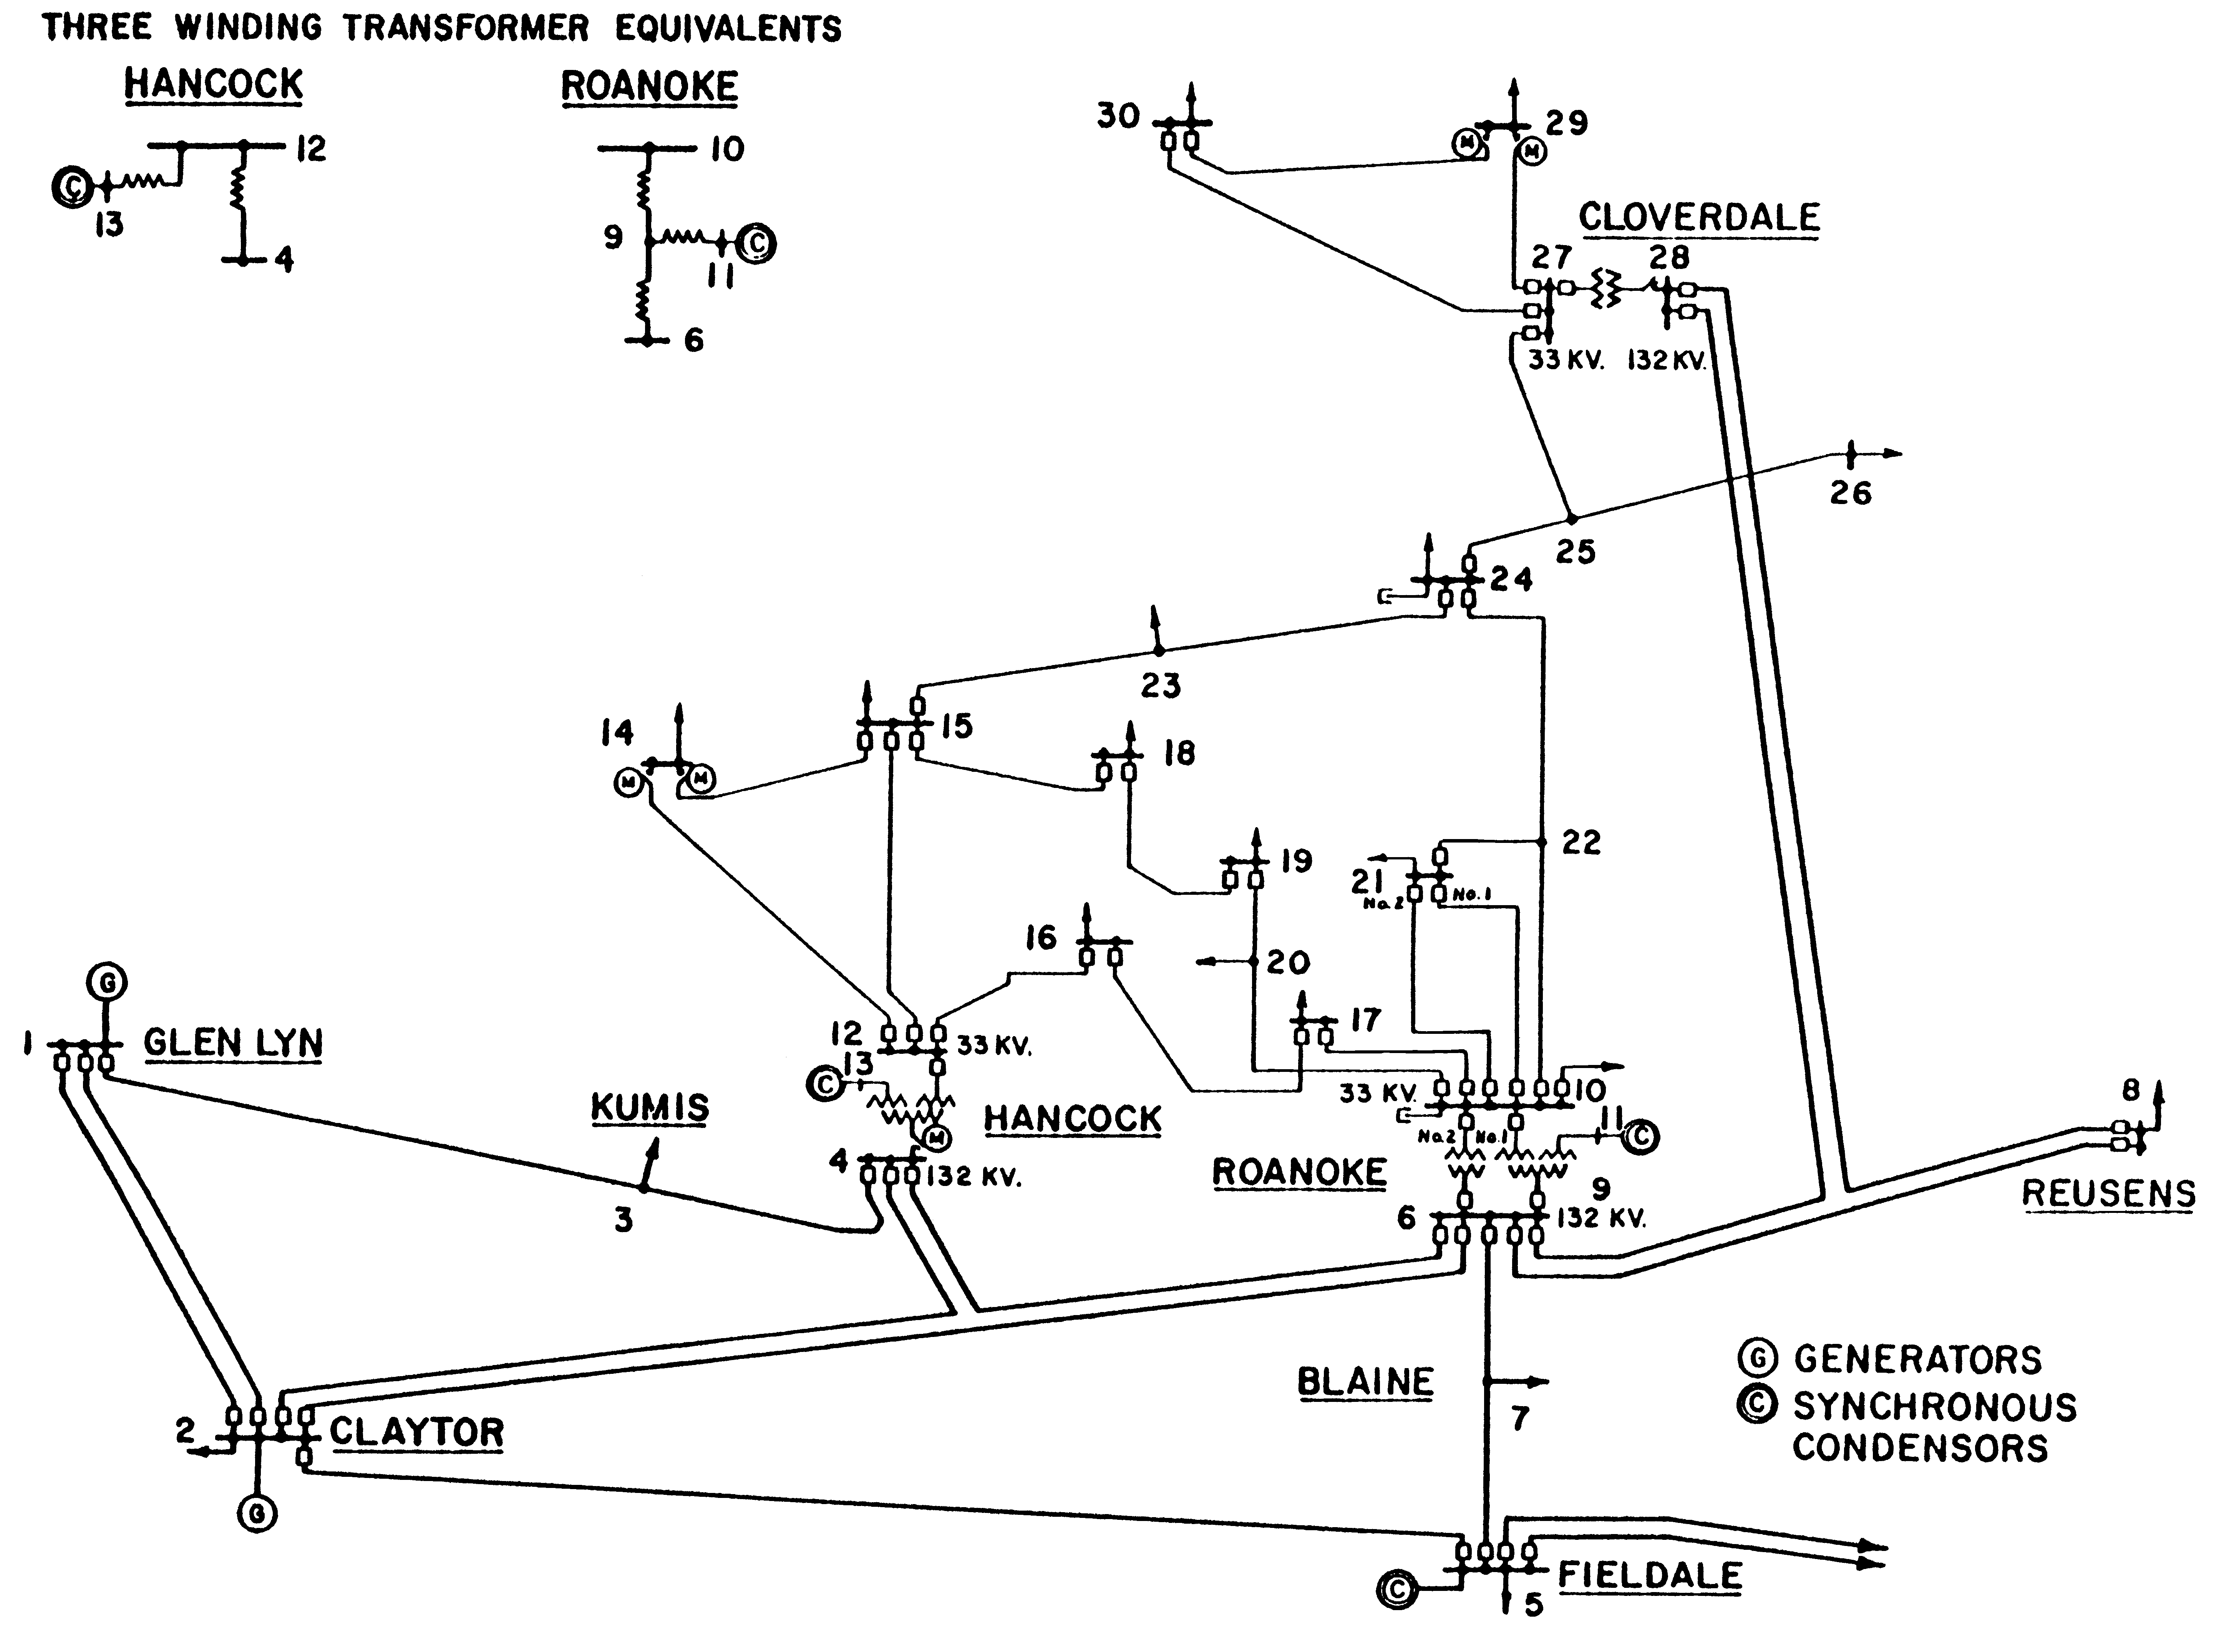
\includegraphics[width=.9\textwidth]{Figures/Lab\ Six/30bus600}
  \caption{The 30-Bus System}
  \label{fig:1}
\end{figure}

\section{Experimentation}

\subsection{Part 1}

We may run the initial contingency case solution to get:

\VerbatimInput{Figures/LabSix/PFOutPartA-b.dat}

\subsection{Contingency Analysis}

\subsubsection{Line 2-5 Outage}

\VerbatimInput[label=Power Flow Solution — Line 2-5 Outage Case]{Figures/LabSix/PFOut2-5.dat}

We may observe that, with a line 2-5 outage, other lines become overloaded in their real power limits. We have two feasible options: we may add shunt capacitors to buses 6/7 to add reactive power or increase line limits. Since shunt capacitors may be expensive to add, we can instead adjust the line limits from $100[\si{\mega\volt\ampere}]\to150[\si{\mega\volt\ampere}]$. This way, the power flow limits are met.

\subsubsection{Line 2-6 Outage}

\VerbatimInput[label=Power Flow Solution — Line 2-6 Outage Case]{Figures/LabSix/PFOut2-6.dat}

We may observe that no contingency correction is needed, as all lines continued to operate despite a loss between lines 2 and 6. Thus, we may leave the system alone.

\subsubsection{Line 15-23 Outage}

\VerbatimInput[label=Power Flow Solution — Line 15-23 Outage Case]{Figures/LabSix/PFOut15-23.dat}

We may observe that no contingency correction is needed, as all lines continued to operate despite a loss between lines 15 and 23. Thus, we may leave the system alone.

\subsubsection{Line 18-19 Outage}

\VerbatimInput[label=Power Flow Solution — Line 18-19 Outage Case]{Figures/LabSix/PFOut18-19.dat}

We may observe that no contingency correction is needed, as all lines continued to operate despite a loss between lines 18 and 19. Thus, we may leave the system alone.

\subsubsection{Line 22-24 Outage}

\VerbatimInput[label=Power Flow Solution — Line 22-24 Outage Case]{Figures/LabSix/PFOut22-24.dat}

We may observe that no contingency correction is needed, as all lines continued to operate despite a loss between lines 22 and 24. We may note that this is because, despite a line limit of $30[\si{\mega\volt\ampere}]$, the shunt capacitor at bus 24 is injecting reactice power to compensate for line overloading. Thus, we may leave the system alone.

\subsubsection{Loss of Synchronous Condeneser (Bus 8)}

\VerbatimInput[label=Power Flow Solution — Loss of Bus 8 Synchronous Condenser]{Figures/LabSix/PFOut8.dat}

The loss of a synchronous condensor means that the bus is unable to adjust the reactive power system as needed. To ensure that the bus is within its reactive limit, we may modify bus 8 such that it is switched from a PV bus to a PQ bus.

\section{Conclusion}

We may observe that outages occurred for only two cases: the outage of line 2/5 and the loss of the synchronous condenser at bus 8. The former resulted in outages due to increased real power flow. We adjusted for this by increasing the line limit from $100\to150[\si{\mega\volt\ampere}]$ (alternatively, we could have added shunt capacitance to buses 6/7. The latter resulted in an inability to adjust for reactive power, and, thus, we changed it from a PV to a PQ bus.

\end{document}
